%\documentclass[11pt,a4paper,oneside,onecolumn]{jarticle}

\documentclass[11pt,a4paper,oneside,onecolumn]{jreport}

\usepackage[dvipdfmx]{graphicx,color}

\usepackage{amsmath,amssymb}
\usepackage{bm}

\usepackage{caption}
\captionsetup[figure]{format=hang, labelformat=simple, labelsep=period, font=small}
\usepackage{here}
\usepackage{chngcntr}
\counterwithin{figure}{section}
\counterwithin{equation}{section}

\usepackage{ascmac}
\usepackage[top=25truemm,bottom=25truemm,left=25truemm,right=25truemm]{geometry}
\usepackage{indentfirst}
\usepackage{fancyhdr}
\pagestyle{fancy}
\lhead{\rightmark}
\cfoot{\thepage}
\setlength{\headheight}{16pt}
\renewcommand{\chaptermark}[1]{\markboth{第\ \normalfont\thechapter\ 章~#1}{}}
\renewcommand{\sectionmark}[1]{\markright{\thesection\ #1}{}}

\usepackage{url}
\usepackage{xcolor}
\usepackage[dvipdfmx,
draft=false,             % /true   hyperrefの全ての機能を無効にする(デフォルトはfalse)
%
bookmarks=true,          % /false  しおりを作るか、否か(デフォルトはtrue)
bookmarksnumbered=true, % /true   しおりに節番号などを付けるか、否か(デフォルトはfalse)
bookmarksopen=false,     % /true   しおりのツリーを開くか、否か(デフォルトはfalse)
bookmarksopenlevel=3,    % しおりの深さ
%
colorlinks=true,         % /true リンクに色をつけるか、否か(デフォルトはfalse)
anchorcolor=black,        % アンカーテキストの色指定(デフォルトはblack)
citecolor=cyan,           % 参考文献リンクの色指定(デフォルトはgreen)
filecolor=magenta,       % ローカルファイルリンクの色指定(デフォルトはmagenta)
linkcolor=cyan,        % 作成しているpdfファイルのリンクの色(デフォルトはred)
linkbordercolor={1 0 0}, % R G B リンクを囲むボックスの色(デフォルトは1 0 0)
urlcolor=blue,         % 外部参照しているurlの色(デフォルトはmagenta)
%
pdfborder={1 1 1},       % 枠なし({0 0 1}デフォルト)
pdftitle={研究メモ},             % pdfのタイトル
pdfauthor={Kazuhide Isoya},            % pdfの著者名
pdfsubject={},           % pdfのサブタイトル
pdfkeywords={研究},          % pdfのキーワード
pdfpagemode=UseThumbs,   % サムネイル表示
]{hyperref}
\usepackage{pxjahyper}%日本語目次


\renewcommand{\bibname}{参考文献}

%%%%%%%%%%%%%%%%%%%%%%%%%%%%%%%%%%%%%%%%%%%%%
\makeatletter

\def\id#1{\def\@id{#1}}
\def\department#1{\def\@department{#1}}
\def\abst#1{
\if@twocolumn
  \twocolumn[
\fi
  \begin{center}
    \let\footnote\thanks
    {\LARGE \bf \@title \par}%
\vspace{5truemm}
  %
%    {\normalsize \@date}%
%    \vskip 0.01em
    {\@department \par} % 所属部分
    {\large\@author\par}
    \vspace{3truemm}
  {\small (\@date)\par} % 提出年月日部分
  \vspace{7truemm}
    \textbf{\large{\bf 概要}}\par
  \begin{quotation}
     {\small  #1}
  \end{quotation}
\end{center}
\par\vskip 1.5em
\if@twocolumn
  ]
\fi
}
\makeatother
%%%%%%%%%%%%%%%%%%%%%%%%%%%%%%%%%%%%%%%%%%%%%
\title{巨大衝突ステージにおける衝突破壊の重要性:\\
$N$体計算$\cdot$統計的手法のハイブリッドコードの開発}
\date{\today}
\department{
名古屋大学大学院 理学研究科 素粒子宇宙物理学専攻\\
理論宇宙物理学研究室 (Ta 研)
}
\author{磯谷和秀}
%%%%%%%%%%%%%%%%%%%%%%%%%%%%%%%%%%%%%%%%%%%%%
\begin{document}
\thispagestyle{plain}
\abst{
太陽系の地球型惑星は、最終段階で火星サイズの原始惑星同士が衝突合体を繰り返し形成される。この巨大衝突ステージにおいて地球や地球-月系が形成される。
一方、太陽系外で起こる巨大衝突ステージは、衝突に伴い放出される破片によりデブリ円盤が形成され、観測されている暖かいデブリ円盤(すなわち地球形成領域のデブリ円盤)を説明することができる\cite{1}。
巨大衝突ステージに形成されるデブリ円盤について調べるためには、原始惑星の長期的軌道進化と、破壊を扱うことができる計算が必要である。
しかし衝突により放出される破片の数は$10^{35}$個以上にもなり、$N$体計算ではとても扱うことはできない。
このような多数の粒子を取り扱うには、一つ一つの粒子を取り扱うのではなく、統計力学に基づいた統計的手法が有効であるが、統計的手法では、破片が重力的に集積する際にサイズ分布が非軸対称になることや、原始惑星による軌道共鳴のような、重力相互作用の取り扱いができない。
すなわち$N$体計算と統計的手法を同時に用いると、軌道進化と破壊を同時に考慮した計算を行うことができる。
そこで本研究では、$N$体計算と統計的手法を組み合わせた、衝突破壊を扱うことができるハイブリッドコードの開発を行う。
多数の破片を少数のトレーサーと呼ばれるスーパー粒子に近似することで$N$体計算のコストを抑える。
またそれぞれのトレーサーの周りに扇形領域\cite{2}を考え、その領域に入った他のトレーサーを用いて表面数密度と平均相対速度を計算し、破壊による天体の減少\cite{3}を取り扱う。
さらに本講演では、ハイブリッドコードにより得られる、巨大衝突ステージにおけるデブリ円盤の明るさの空間分布進化についても議論する。
}
\clearpage

\tableofcontents
\clearpage

\chapter{研究メモ}

\section{テスト計算}


\begin{figure}[H]
 \centering
 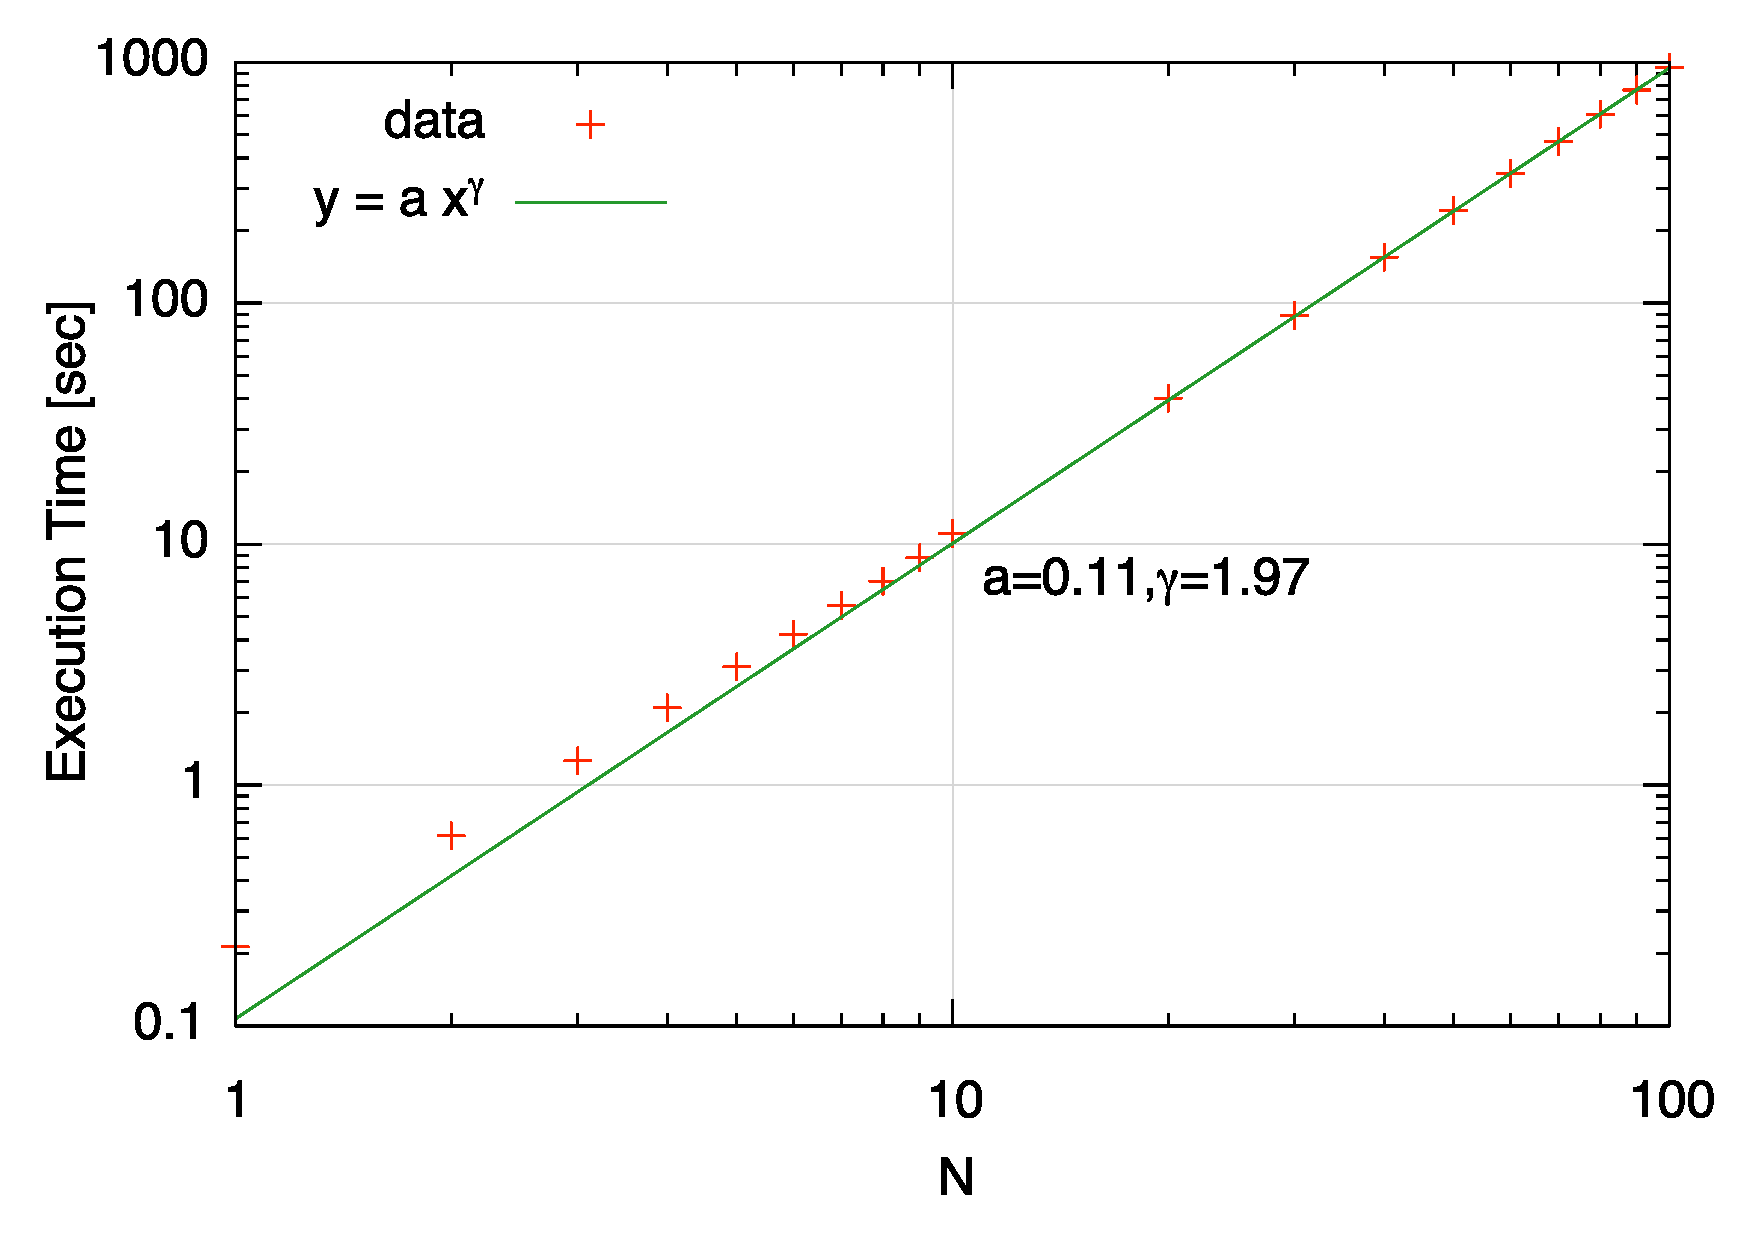
\includegraphics[width=12cm]{./image/ExecutionTime_NoFrag.pdf}
 \caption{微惑星の数と計算実行時間の関係.太陽から $0.95 - 1.05 {\rm AU}$ の位置に質量 $1 \times 10^{24} {\rm g}$ の微惑星を $N$ 個一様に配置し,微惑星同士の相互重力計算を含めて $1000$ 年分計算を行った.赤色の点はデータをプロットしたものであり,緑色の線はデータを $y = a x^{\gamma}$ でフィッティングした曲線である.\label{}}
\end{figure}


\begin{figure}[H]
 \centering
 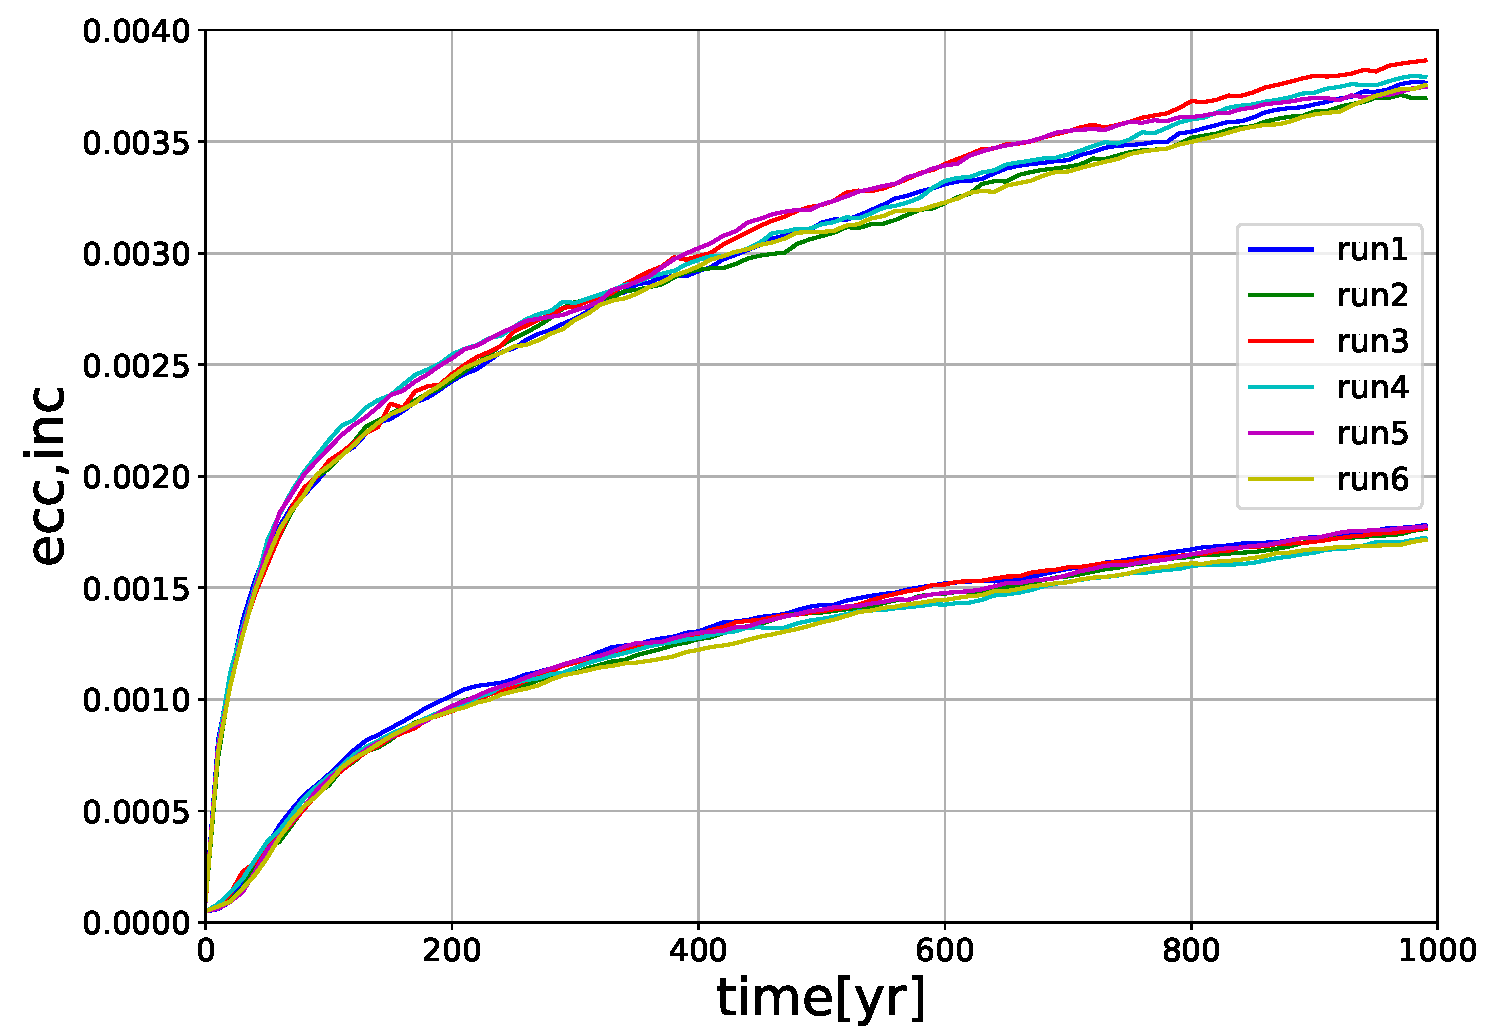
\includegraphics[width=12cm]{./image/Nbodytest_figa_6run.pdf}
 \caption{微惑星の離心率$\cdot$軌道傾斜角の二乗平均平方根の時間進化.太陽から $1 {\rm AU}$ の位置に質量 $1 \times 10^{24} {\rm g}$ の微惑星を $1000$ 個配置し,$1000$ 年分計算を6回行った.ここで,初期の微惑星の面密度が $10 {\rm g/cm^2}$ となるように,$0.965 - 1.035 {\rm AU}$ に一様に配置した.また,初期の離心率$\cdot$軌道傾斜角はレイリー分布に従い,それぞれの二乗平均平方根は $e_{\rm RMS} = 1 \times 10^{-4}, i_{\rm RMS} = 5 \times 10^{-5}$ とした.\label{}}
\end{figure}


\begin{figure}[H]
 \centering
 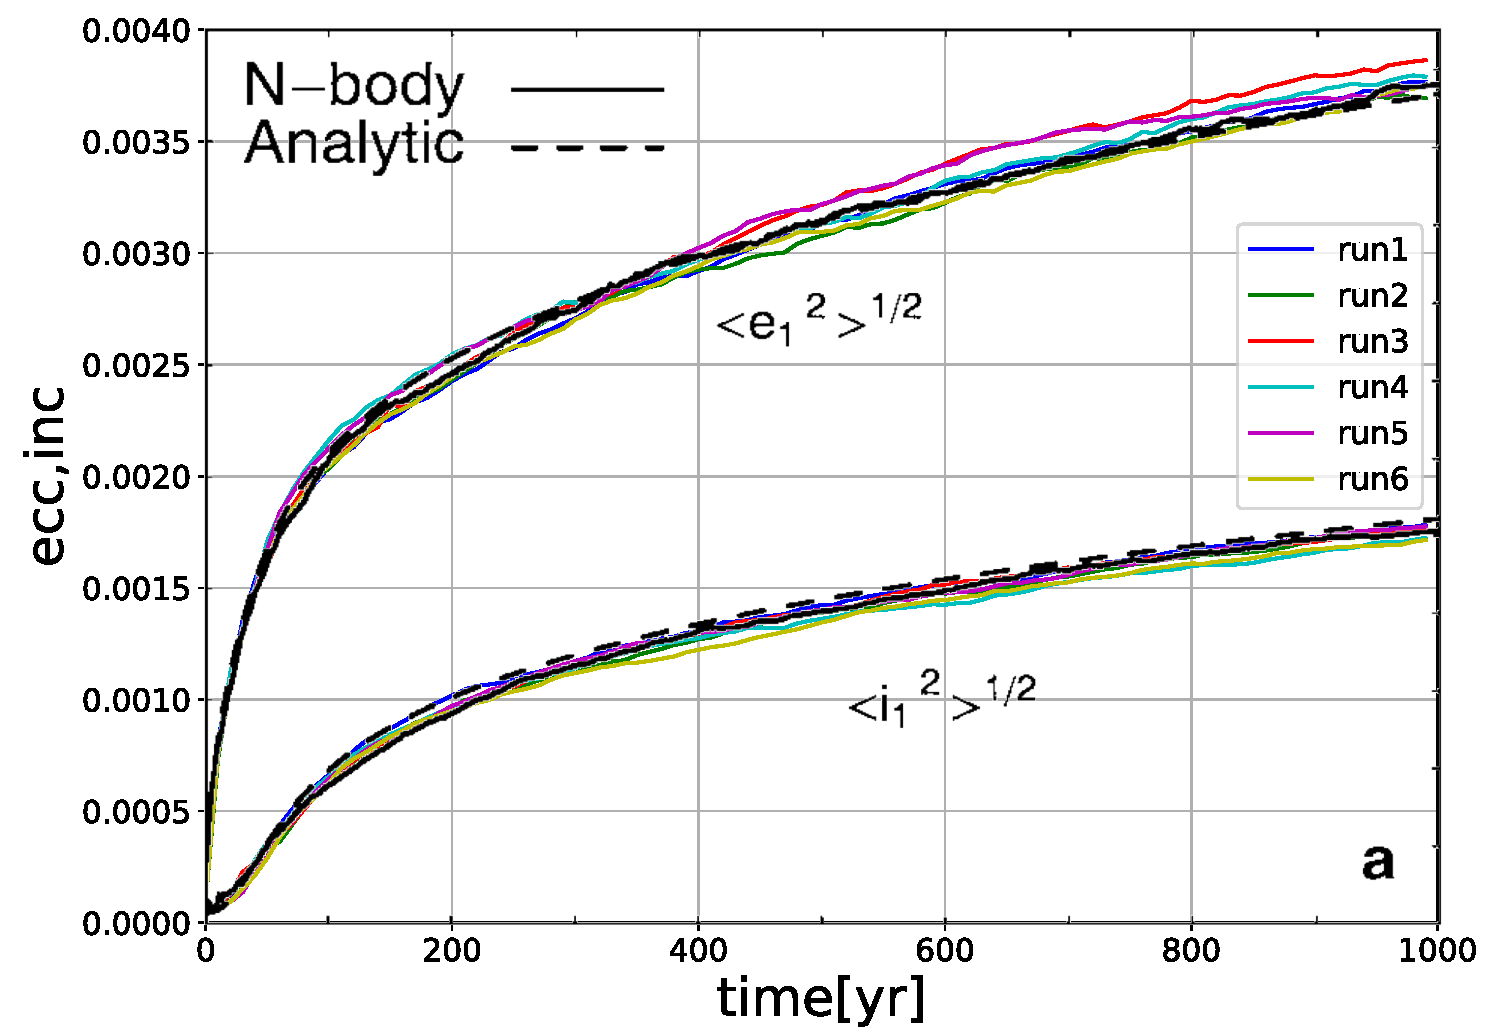
\includegraphics[width=12cm]{./image/Ohtsuki_figa_and_Nbodytest_6run.pdf}
 \caption{Otsuki et al.(2002)のFig.4aとの比較.\label{}}
\end{figure}


\begin{figure}[H]
 \centering
 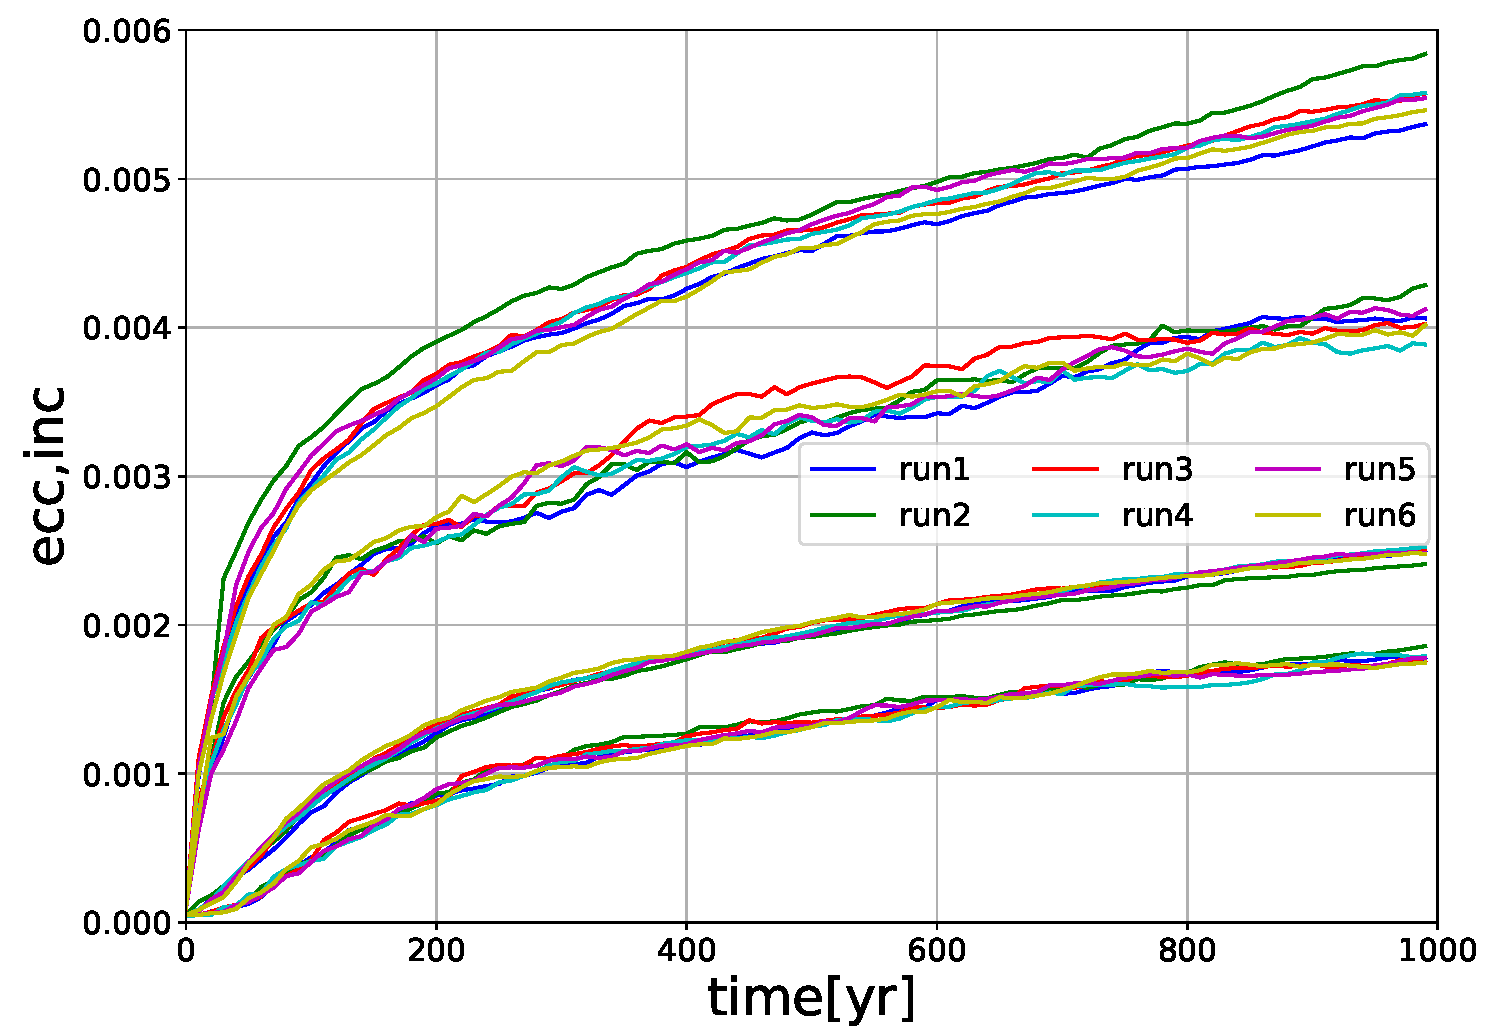
\includegraphics[width=12cm]{./image/Nbodytest_figb_6run.pdf}
 \caption{小さい微惑星と大きい微惑星が混在するときの離心率$\cdot$軌道傾斜角の二乗平均平方根の時間進化.太陽から $1 {\rm AU}$ の位置に質量 $1 \times 10^{24} {\rm g}$ の微惑星を $800$ 個,$4 \times 10^{24} {\rm g}$ の微惑星を $200$ 個配置し,$1000$ 年分計算を6回行った.ここで,初期の微惑星の面密度が $10 {\rm g/cm^2}$ となるように,$0.943 - 1.057 {\rm AU}$ に一様に配置した.また,初期の離心率$\cdot$軌道傾斜角はレイリー分布に従い,それぞれの二乗平均平方根は $e_{\rm RMS} = 1 \times 10^{-4}, i_{\rm RMS} = 5 \times 10^{-5}$ とした.\label{}}
\end{figure}


\begin{figure}[H]
 \centering
 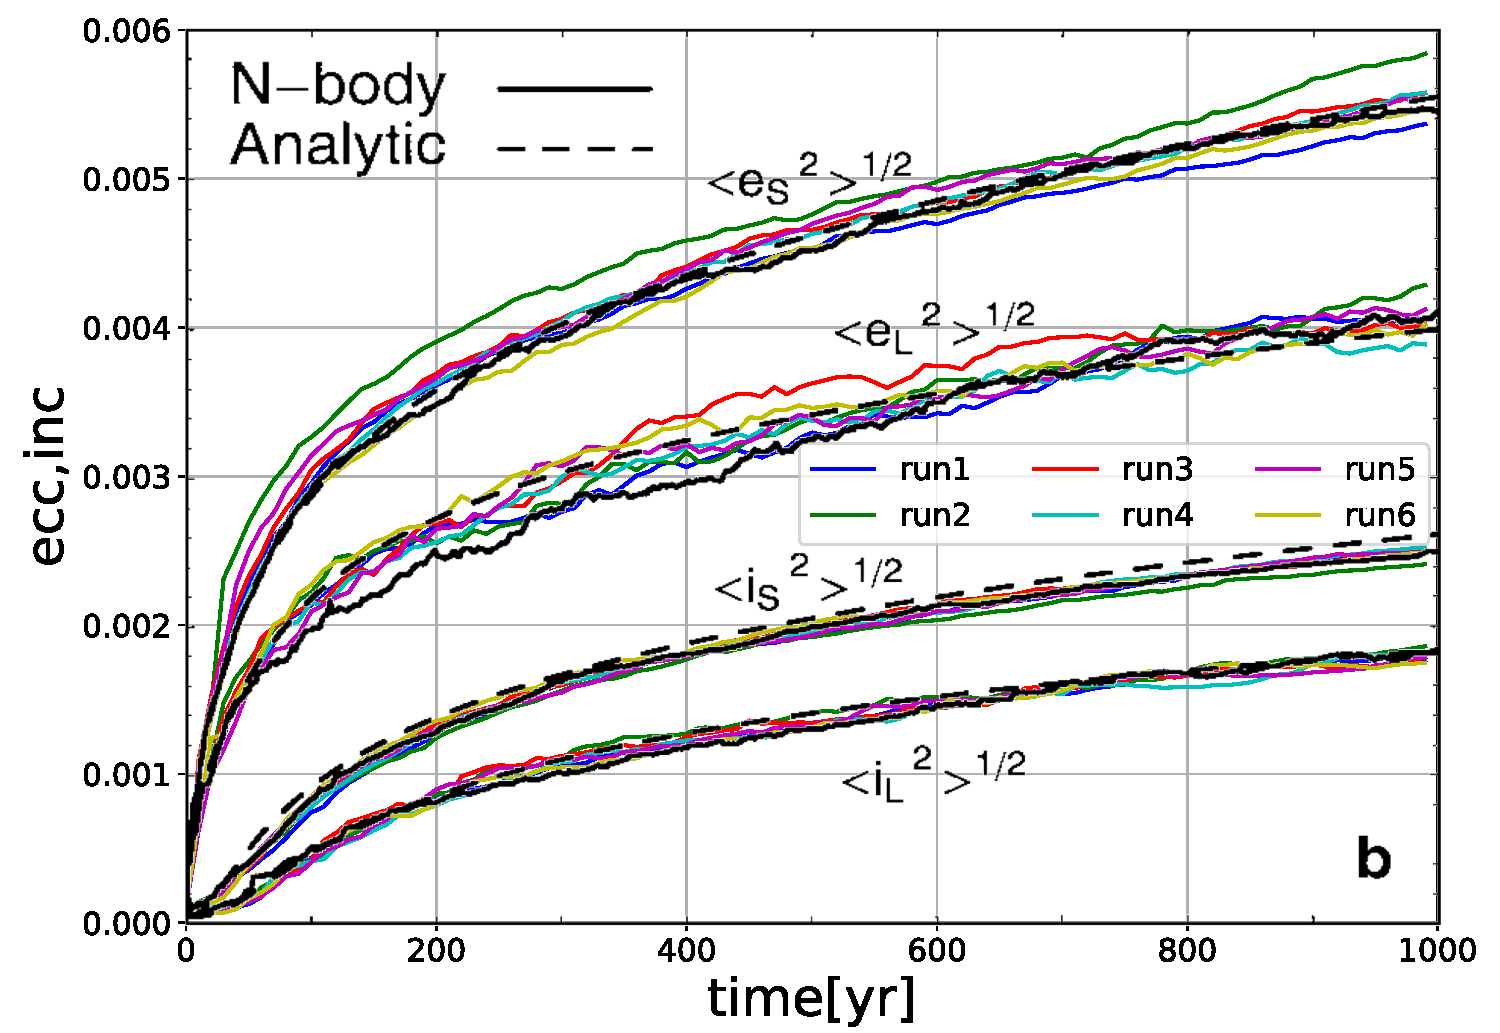
\includegraphics[width=12cm]{./image/Ohtsuki_figb_and_Nbodytest_6run.pdf}
 \caption{Otsuki et al.(2002)のFig.4bとの比較.\label{}}
\end{figure}


\begin{figure}[H]
 \centering
 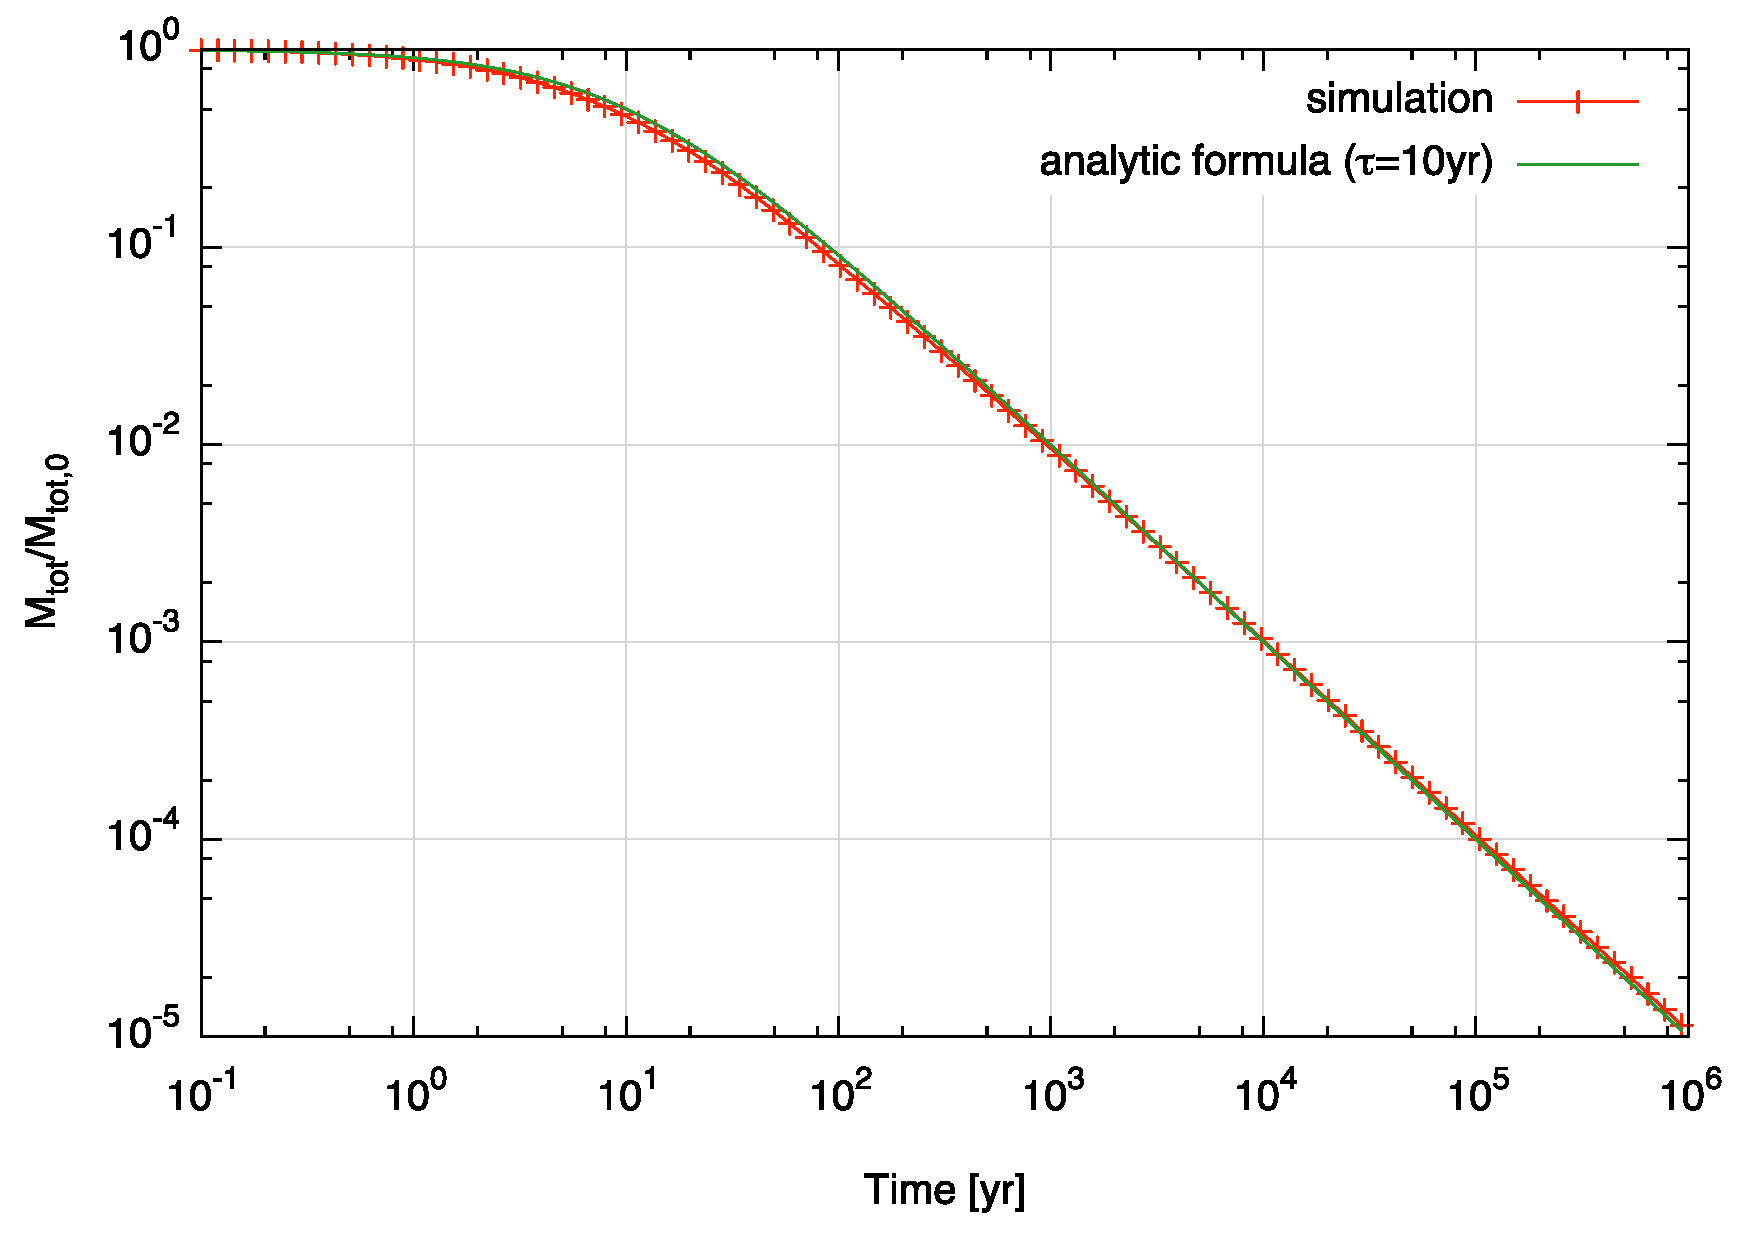
\includegraphics[width=12cm]{./image/MassDepletion_NoInteraction_1Myr.pdf}
 \caption{統計的手法を用いたときの微惑星総質量の時間進化.扇形領域の大きさを決める $\Delta r$ を $0.25 {\rm AU}$ で固定している.太陽から $0.95 - 1.05 {\rm AU}$ の位置に等質量のトレーサーを $100$ 個一様に配置し,$10^6$ 年分計算を行った.ここで,トレーサー同士の相互重力は計算しておらず,トレーサーの軌道要素は変化していない.すべてのトレーサーは初期に離心率 $e = 0.01$,軌道傾斜角 $i = 0.005$ をもち,その他の角変数はランダムで与えた.質量減少タイムスケール $\tau$ が $10$ 年となるように,初期の総質量を $9.92 \times 10^{29} {\rm g}$ とし,解析解の表式\cite{3}と比較した.\label{}}
\end{figure}


\begin{figure}[H]
 \centering
 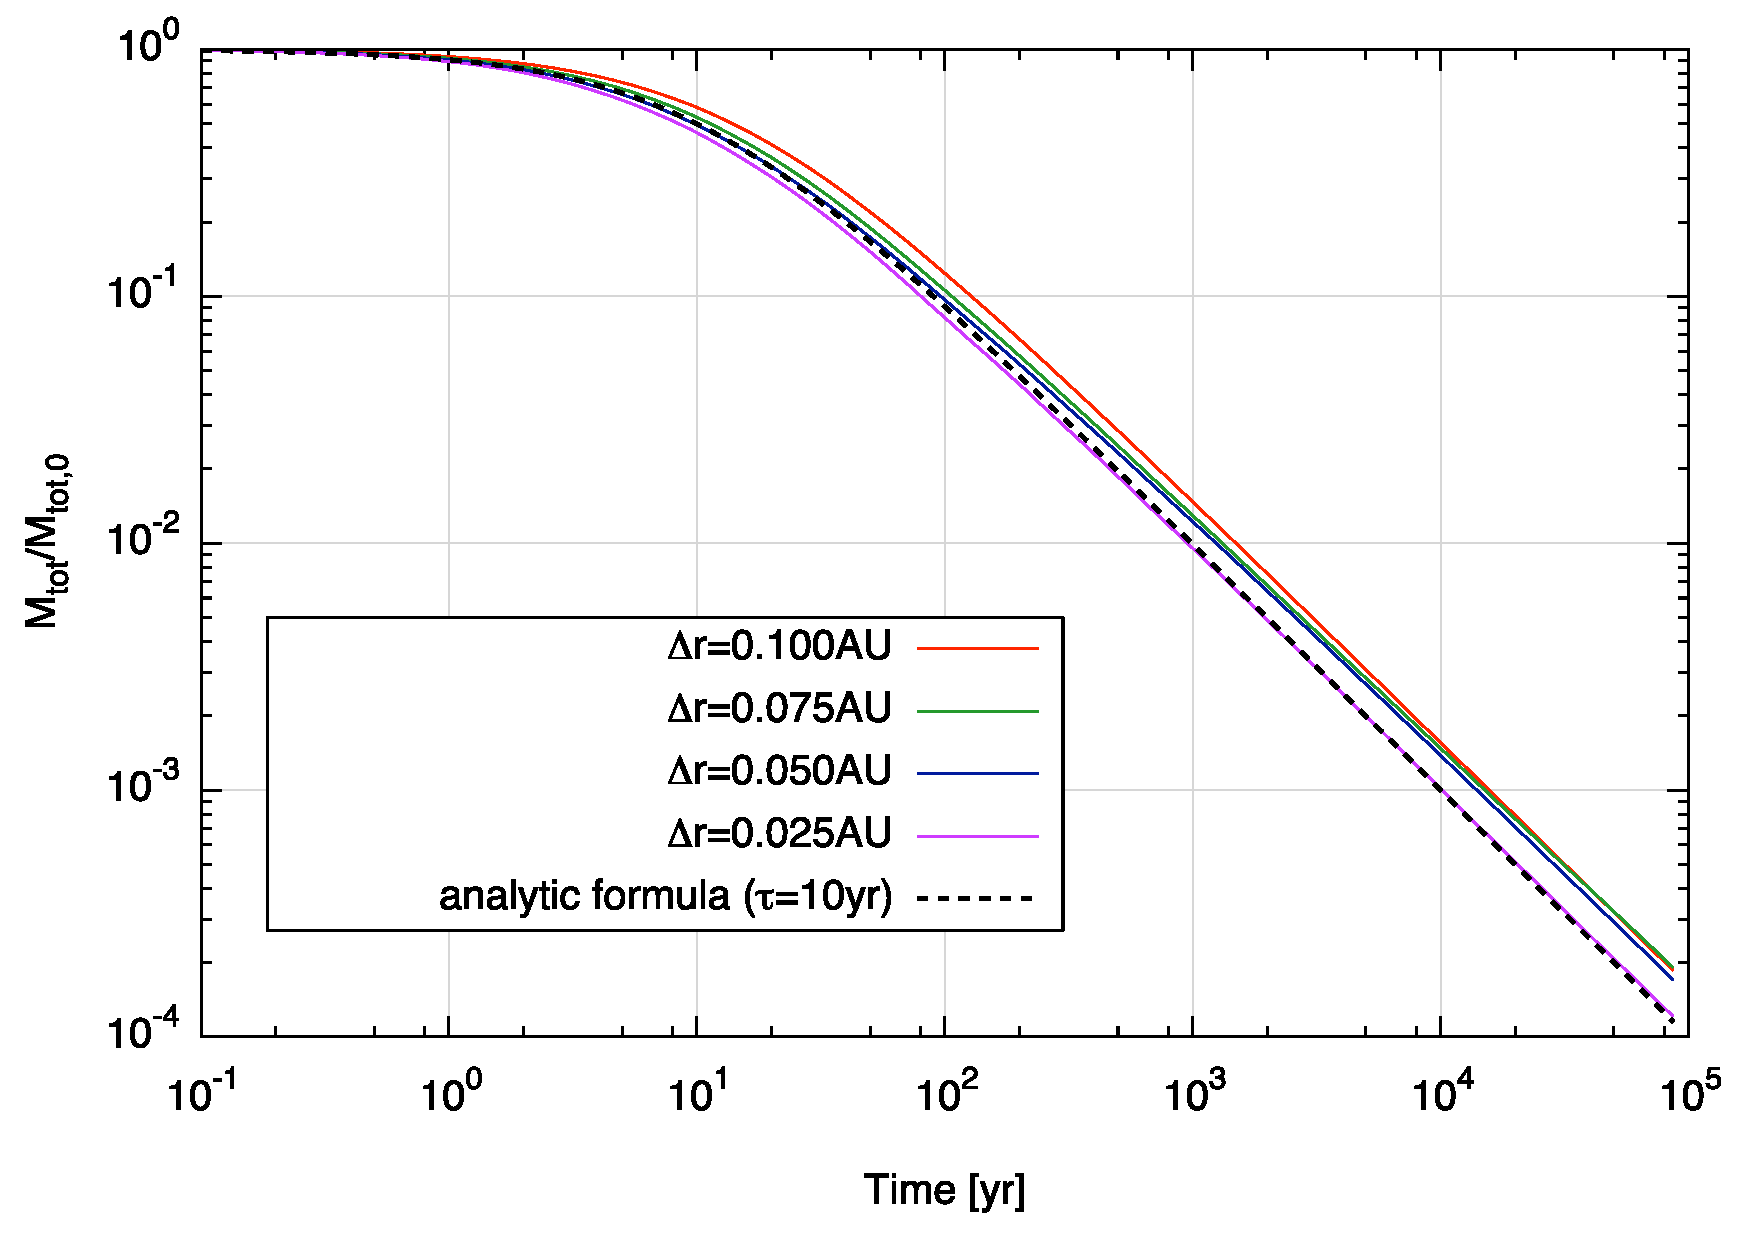
\includegraphics[width=12cm]{./image/MassDepletion_NoInteraction_100kyr.pdf}
 \caption{統計的手法を用いたときの微惑星総質量の時間進化.扇形領域の大きさを決める $\Delta r$ を,$0.1,0.075,0.05,0.025 {\rm AU}$ で固定している.太陽から $0.95 - 1.05 {\rm AU}$ の位置に等質量のトレーサーを $100$ 個一様に配置し,$10^5$ 年分計算を行った.ここで,トレーサー同士の相互重力は計算しておらず,トレーサーの軌道要素は変化していない.すべてのトレーサーは初期に離心率 $e = 0.01$,軌道傾斜角 $i = 0.005$ をもち,その他の角変数はランダムで与えた.質量減少タイムスケール $\tau$ が $10$ 年となるように,初期の総質量を $9.92 \times 10^{29} {\rm g}$ とし,解析解の表式\cite{3}と比較した.\label{}}
\end{figure}


\begin{figure}[H]
 \centering
 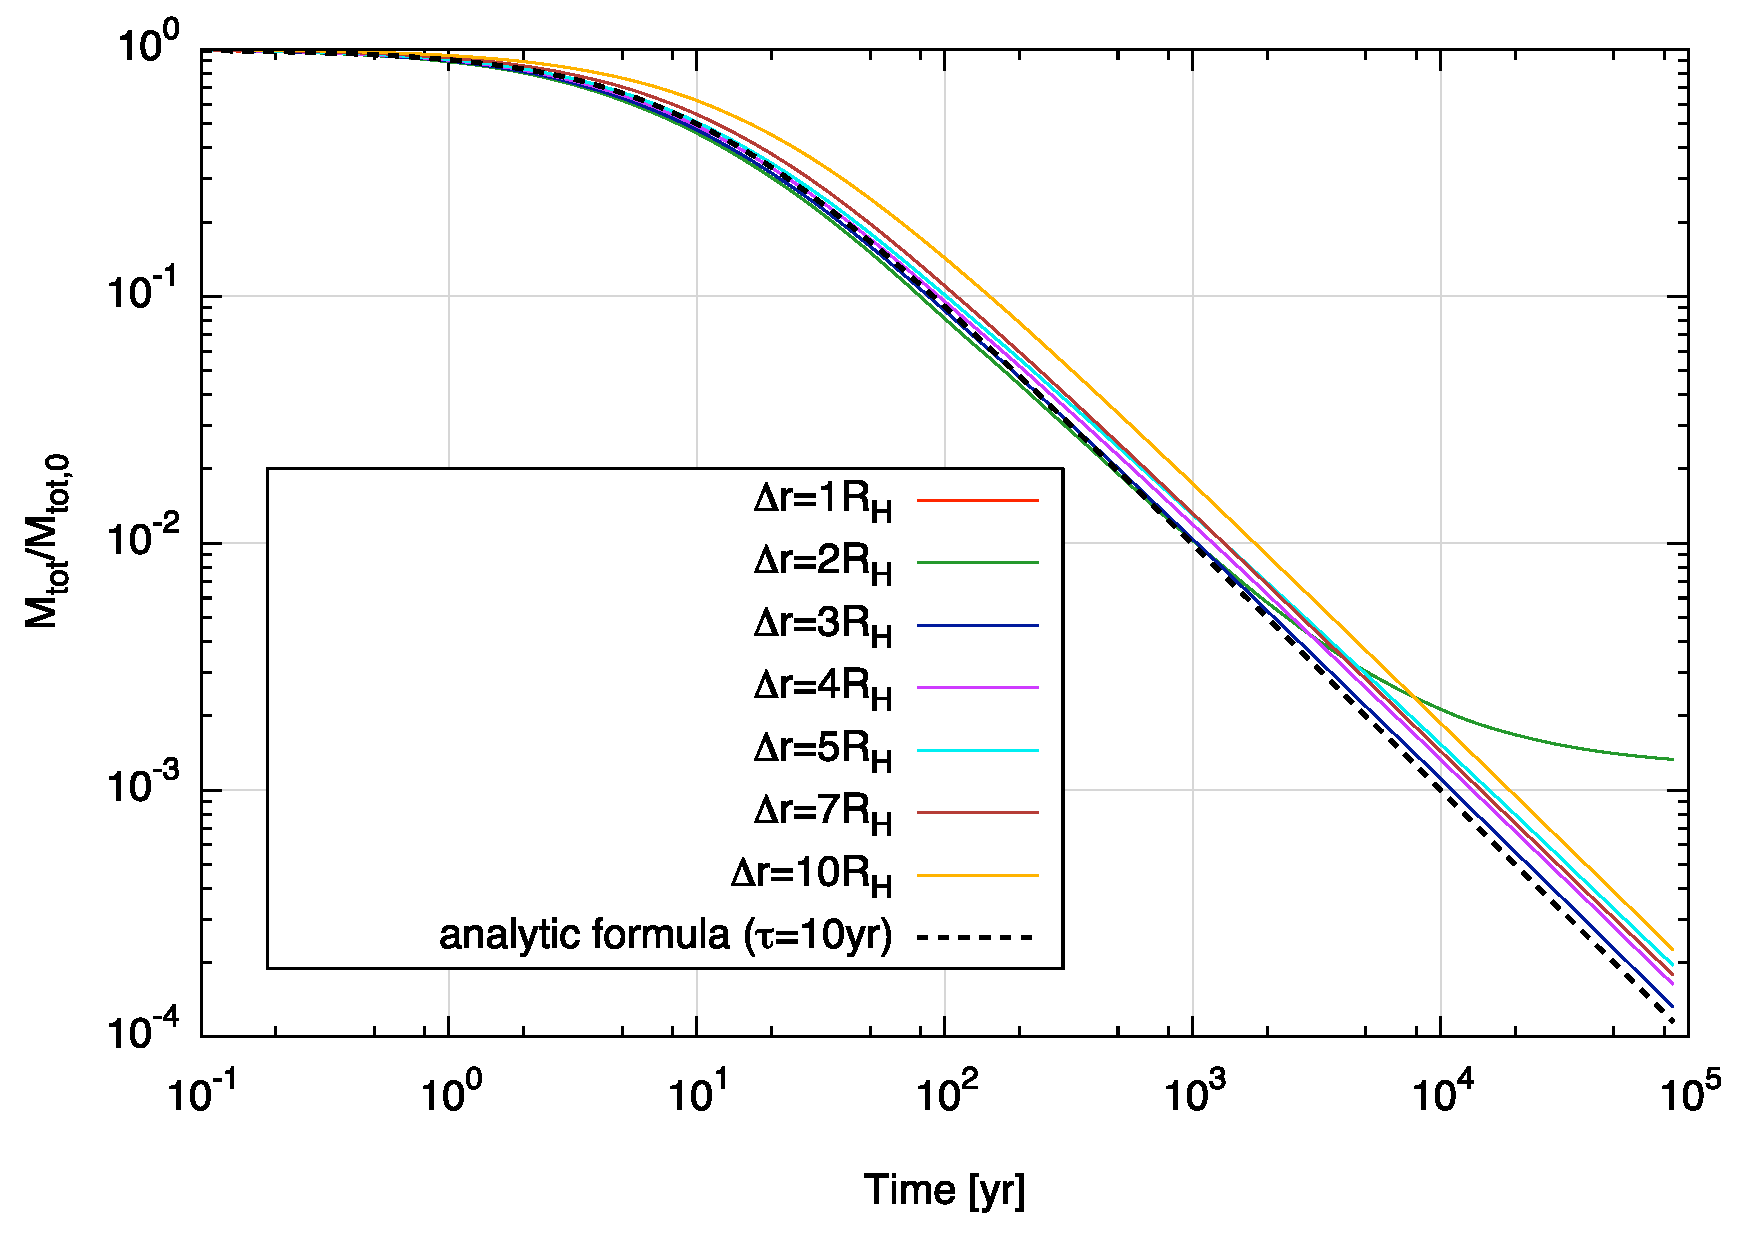
\includegraphics[width=12cm]{./image/MassDepletion_NoInteraction_2_100kyr.pdf}
 \caption{統計的手法を用いたときの微惑星総質量の時間進化.扇形領域の大きさを決める $\Delta r$ を,$1,2,3,5,7,10 {\rm R_H}$ で固定している.太陽から $0.95 - 1.05 {\rm AU}$ の位置に等質量のトレーサーを $100$ 個一様に配置し,$10^5$ 年分計算を行った.ここで,トレーサー同士の相互重力は計算しておらず,トレーサーの軌道要素は変化していない.すべてのトレーサーは初期に離心率 $e = 0.01$,軌道傾斜角 $i = 0.005$ をもち,その他の角変数はランダムで与えた.質量減少タイムスケール $\tau$ が $10$ 年となるように,初期の総質量を $9.92 \times 10^{29} {\rm g}$ とし,解析解の表式\cite{3}と比較した.\label{}}
\end{figure}



\appendix
\chapter{論文}

\section{Kobayashi \& Tanaka 2010 数式}


\begin{align}
 &\frac{\partial m n_{\rm s}(m)}{\partial t} + \frac{\partial F(m)}{\partial m} = 0\\
 &\Omega_{\rm K} n_{\rm s} (m_1) d m_1 n_{\rm s} (m_2) d m_2 P_{\rm col}\\
 &P_{\rm col} = \pi (r_1 + r_2)^2 \frac{{\cal F} (I)}{2 \pi^2} = h_0 m_1^{\frac{2}{3}} (1 + y^{\frac{1}{3}})^2\\
 &h_0 = 6.1 \times 10^{-2} {\cal F} (I) \rho ^{- \frac{2}{3}}\\
 &m_1 f (m, m_1, m_2)\\
 &m_2 f (m, m_2, m_1)\\
 &\frac{1}{m} \frac{\partial}{\partial m} [m_1 f (m, m_1, m_2) + m_2 f (m, m_2, m_1)] dm\\
 &F (m) = - \int_m^{\infty} d m_1 \int_0^{\infty} d m_2 \Omega_{\rm K} m_1 f(m, m_1, m_2) P_{\rm col} n_{\rm s} (m_1) n_{\rm s} (m_2)\\
 &\phi (y) = \frac{E_{\rm imp}}{m_1 Q_{\rm D}^{\ast}} = \frac{v^2}{2 Q_{\rm D}^{\ast}} \frac{y}{1 + y}\\
 &E_{\rm imp} = \frac{1}{2} \frac{m_1 m_2}{m_1 + m_2} v^2\\
 &m_{\rm e} = \frac{\phi}{1 + \phi} m_1\\
 &m_{\rm L} = \frac{\epsilon}{1 + \phi} m_{\rm e} = \frac{\epsilon \phi}{(1 + \phi)^2} m_1\\
 &f (m, m_1, m_2) = f_{\rm eject} (m, m_1, m_2) + f_{\rm rem} (m, m_1, m_2)\\
 &m_1 f_{\rm eject} (m, m_1, m_2) = \left\{
 \begin{array}{ll}
  m_{\rm e} & (m>m_{\rm L})\\
  m_{\rm e} \left( \frac{m}{m_{\rm L}} \right)^{2-b} & (m \leq m_{\rm L})\\
 \end{array}
 \right.\\
 &m_1 f_{\rm rem} (m, m_1, m_2) = \left\{
 \begin{array}{ll}
  m_1 - m_{\rm e} & (m \geq m_1 - m_{\rm e})\\
  0 & (m < m_1 - m_{\rm e})\\
 \end{array}
 \right.\\
 &\frac{v^2}{Q_{\rm D}^{\ast}} \sim 2 \times 10^2 \left( \frac{e}{0.1} \right)^2 \left( \frac{a}{50\ {\rm AU}} \right)^{-1} \left( \frac{M_{\ast}}{{\rm M_{\odot}}} \right) \left( \frac{Q_{\rm D}^{\ast}}{10^7\ {\rm erg/g}} \right)^{-1}\\
 &f (m, m_1, m_2) = f \left( \frac{m}{m_1}, \frac{m_2}{m_1} \right)
\end{align}
 
\begin{align}
 &n_{\rm s} (m) = A m^{- \alpha}\\
 &F (m) = - A^2 \Omega_{\rm K} h_0 m^{\frac{11}{3} - 2 \alpha} \int_0^1 dx \int_0^{\infty} dy y^{-\alpha} \left( 1 + y^{\frac{1}{3}} \right)^2 x^{2 \alpha - \frac{14}{3}} f(x, y)\\
 &\frac{\partial F(m)}{\partial m} = 0\\ 
 &\alpha = \frac{11}{6}\\
 &F(m) = F_{\rm eject}(m) + F_{\rm rem}(m)\\
 F_{\rm eject}(m) = & - A^2 \Omega_{\rm K} h_0 \int_0^{\infty} dy \frac{y^{- \alpha} \left( 1 + y^{\frac{1}{3}} \right)^2 \phi(y)}{1 + \phi(y)}\\
 &\times \left\{ \int_0^{k(y)} x^{2 \alpha - \frac{14}{3}}\left[ \frac{x}{k(y)} \right]^{2-b} dx + \int_{k(y)}^1 x^{2 \alpha - \frac{14}{3}} dx \right\}\\
 F_{\rm rem}(m) = & - A^2 \Omega_{\rm K} h_0 \int_0^{\infty} dy \frac{y^{- \alpha} \left( 1 + y^{\frac{1}{3}} \right)^2}{1 + \phi(y)} \int_{\frac{1}{1 + \phi(y)}}^1 x^{2 \alpha - \frac{14}{3}} dx\\
 &k(y) = \frac{\epsilon \phi(y)}{\left[ 1 + \phi(y) \right]^2}\\
 F_{\rm eject}(m) = & - A^2 \Omega_{\rm K} h_0 \int_0^{\infty} dy \frac{y^{- \alpha} \left( 1 + y^{\frac{1}{3}} \right)^2 \phi(y)}{1 + \phi(y)}\\
 &\times \left[ - \ln \frac{\epsilon \phi(y)}{\left[ 1 + \phi(y) \right]^2} + \frac{1}{2 - b} \right]\\
 F_{\rm rem}(m) = & - A^2 \Omega_{\rm K} h_0 \int_0^{\infty} dy \frac{y^{- \alpha} \left( 1 + y^{\frac{1}{3}} \right)^2}{1 + \phi(y)} \ln \left( 1 + \phi(y) \right)\\
 &F(m) \propto \left\{
 \begin{array}{ll}
  \left(\frac{v^2}{Q_{\rm D}^{\ast}}\right) \ln \left(\frac{v^2}{Q_{\rm D}^{\ast}}\right) & {\rm for}\ \frac{v^2}{Q_{\rm D}^{\ast}} \ll 1\\
  \left(\frac{v^2}{Q_{\rm D}^{\ast}}\right)^{\alpha - 1} & {\rm for}\ \frac{v^2}{Q_{\rm D}^{\ast}} \gg 1\\
 \end{array}
 \right.\\
 &F'(m, y') = F'_{\rm eject} (m, y') + F'_{\rm rem} (m, y')\\
 F'_{\rm eject}(m, y') = & - A^2 \Omega_{\rm K} h_0 \int_0^{y'} dy \frac{y^{- \alpha} \left( 1 + y^{\frac{1}{3}} \right)^2 \phi(y)}{1 + \phi(y)}\\
 &\times \left[ - \ln \frac{\epsilon \phi(y)}{\left[ 1 + \phi(y) \right]^2} + \frac{1}{2 - b} \right]\\
 F'_{\rm rem}(m, y') = & - A^2 \Omega_{\rm K} h_0 \int_0^{y'} dy \frac{y^{- \alpha} \left( 1 + y^{\frac{1}{3}} \right)^2}{1 + \phi(y)} \ln \left( 1 + \phi(y) \right)\\
 &F(m) = - A^2 \Omega_{\rm K} h_0 \left( \frac{v^2}{Q_{\rm D}^{\ast}} \right)^{\frac{5}{6}} \left[ \left( - \ln \epsilon + \frac{1}{2 - b} \right) s_1 + s_2 + s_3 \right]\\
 &\phi(y) \sim 1\\
 &y \ll 1
\end{align}

\begin{align}
 &\int_0^{\infty} dy \frac{y^{- \alpha} \left( 1 + y^{\frac{1}{3}} \right)^2 \phi(y)}{1 + \phi(y)} \left[ - \ln \frac{\epsilon \phi(y)}{\left[ 1 + \phi(y) \right]^2} + \frac{1}{2 - b} \right]\\
 &+ \int_0^{\infty} dy \frac{y^{- \alpha} \left( 1 + y^{\frac{1}{3}} \right)^2}{1 + \phi(y)} \ln \left( 1 + \phi(y) \right)\\
 \approx& \left(\frac{v^2}{2Q_{\rm D}^{\ast}}\right)^{\alpha - 1} \int_0^{\infty} d \phi \left\{ \frac{\phi^{1 - \alpha}}{1 + \phi} \left[ - \ln \frac{\epsilon \phi}{\left(1 + \phi\right)^2} + \frac{1}{2 - b} \right] + \frac{\phi^{- \alpha}}{1 + \phi} \ln \left(1 + \phi \right) \right\}\\
 =& \left(\frac{v^2}{2Q_{\rm D}^{\ast}}\right)^{\alpha - 1} \left[ \left(- \ln \epsilon + \frac{1}{2 - b} \right) s_1(\alpha) + s_2(\alpha) + s_3(\alpha) \right]\\
 &s_1(\alpha) = \int_0^{\infty} d \phi \frac{\phi^{1 - \alpha}}{1 + \phi}\\
 &s_2(\alpha) = - \int_0^{\infty} d \phi \frac{\phi^{1 - \alpha}}{1 + \phi} \ln \frac{\phi}{\left(1 + \phi \right)^2}\\
 &s_3(\alpha) = \int_0^{\infty} d \phi \frac{\phi^{1 - \alpha}}{1 + \phi} \ln (1 + \phi)\\
 &\frac{d \Sigma}{d t} = F(m)\\
 &\Sigma = \int_{m_{\rm min}}^{m_{\rm max}} m n_{\rm s} dm = \frac{m_{\rm max}^{2 - \alpha}}{2 - \alpha} A\\ 
 &\Sigma(t) = \frac{\Sigma_0}{1 + t/\tau_{\rm dep}}\\
 \tau_{\rm dep}^{-1} =& \frac{1}{36}\Omega_{\rm K}\frac{\Sigma_0}{m_{\rm max}}h_0 m_{\rm max}^{\frac{2}{3}}\\
 &\times \left\{ \int_0^{\infty} dy \frac{y^{-\alpha}\left(1 + y^{\frac{1}{3}}\right)^2\phi(y)}{1 + \phi(y)} \left[ - \ln \left( \frac{\epsilon\phi(y)}{\left[1 + \phi(y)\right]^2} \right) + \frac{1}{2 - b} \right] \right.\\
 &\left. \ \ \ \ + \int_0^{\infty} dy \frac{y^{- 
\alpha}\left(1 + y^{\frac{1}{3}}\right)^2}{1 + \phi(y)} \ln \left( 1 + \phi(y) \right) \right\}\\
 &\tau_{\rm dep} = \frac{36 m_{\rm max}^{\frac{1}{3}}}{\Sigma_0h_0\Omega_{\rm K}} \left( \frac{v^2}{2Q_{\rm D}^{\ast}} \right)^{- \frac{5}{6}} \left[ \left(- \ln \epsilon + \frac{1}{2 - b} \right) s_1 + s_2 + s_3 \right]^{-1}\\
 F(m) =& - A^2 \Omega_{\rm K} h_0 m^{\frac{11}{3} - 2 \alpha} \left( \frac{v(m)^2}{Q_{\rm D}^{\ast}(m)} \right)^{\alpha - 1}\\
 &\times \left[ \left( - \ln \epsilon + \frac{1}{2 - b} \right) s_1(\alpha) + s_2(\alpha) + s_3(\alpha) \right]\\
 &\frac{v(m)^2}{Q_{\rm D}^{\ast}(m)} \propto m^{-p}\\ 
 &\frac{11}{3}-2\alpha-p(\alpha-1) = 0\\
 &\alpha = \frac{11+3p}{6+3p}
\end{align}

\begin{align}
 \tau_{\rm dep} =& \frac{m_{\rm max}^{\frac{1}{3}}}{(2-\alpha)^2\Sigma_0h_0\Omega_{\rm K}} \left( \frac{v(m_{\rm max})^2}{2Q_{\rm D}^{\ast}(m_{\rm max})} \right)^{-\alpha+1}\\
 &\times \left[ \left(- \ln \epsilon + \frac{1}{2 - b} \right) s_1(\alpha) + s_2(\alpha) + s_3(\alpha) \right]^{-1}\\
 &Q_{\rm D}^{\ast} = Q_0 \left( \frac{\rho}{3\ {\rm g cm^{-3}}} \right)^{0.55} \left( \frac{m}{10^{21}\ {\rm g}} \right)^{0.45}\ {\rm erg/g}\\
 &v = e v_{\rm K}\\
 \tau_{\rm dep} =& 2.0 \times 10^{10}f \left( \frac{Q_0}{9.5 \times 10^8\ {\rm erg/g}} \right)^{0.68} \left( \frac{m}{10^{21}\ {\rm g}} \right)^{0.64} \left( \frac{a}{50\ {\rm AU}} \right)^{4.18}\\
 &\times \left( \frac{\Delta a/a}{0.1} \right) \left( \frac{e}{0.1} \right)^{-1.4} \left( \frac{\rho}{3\ {\rm g cm^{-3}}} \right)^{0.89} \left( \frac{M_{\rm tot}}{{\rm M_{\oplus}}} \right)^{-1}\ {\rm yr}\\
 &{\rm M_{\oplus}} = 5.97 \times 10^{27}\ {\rm g}\\
 \tau_{\rm grow} =& 2.9 \times 10^6 \left( \frac{m}{10^{21}\ {\rm g}} \right)^{1/9} \left( \frac{a}{5.2\ {\rm AU}} \right)^{1/6} \left( \frac{\rho_{\rm gas}}{10^{-9}\ {\rm g cm^{-3}}} \right)^{-1/3}\\
 &\times \left( \frac{\rho}{3\ {\rm g cm^{-3}}} \right)^{5/9} \left( \frac{M}{10^{26}\ {\rm g}} \right)^{1/3} \left( \frac{\Sigma}{2.5\ {\rm g cm^{-2}}} \right)^{-1}\ {\rm yr}\\
 \tau_{\rm dep} =& 8.9 \times 10^6 \left( \frac{Q_0}{9.5 \times 10^8\ {\rm erg/g}} \right)^{0.69} \left( \frac{a}{5.2\ {\rm AU}} \right)^{2.4} \left( \frac{\rho_{\rm gas}}{10^{-9}\ {\rm g cm^{-3}}} \right)^{0.23}\\
 &\times \left( \frac{m}{10^{21}\ {\rm g}} \right)^{0.57} \left( \frac{M}{10^{26}\ {\rm g}} \right)^{-0.46} \left( \frac{\rho}{3\ {\rm gcm^{-3}}} \right)^{0.89} \left( \frac{\Sigma}{2.5\ {\rm g cm^{-2}}} \right)^{-1}\ {\rm yr}\\
 M =& 6.7 \times 10^{-2} \left( \frac{Q_0}{9.5 \times 10^8\ {\rm erg/g}} \right)^{0.87} \left( \frac{m}{10^{21}\ {\rm g}} \right)^{0.58}\\ 
 &\times \left( \frac{a}{5.2\ {\rm AU}} \right)^{2.8} \left( \frac{\rho_{\rm gas}}{10^{-9}\ {\rm g cm^{-3}}} \right)^{0.71} \left( \frac{\rho}{3\ {\rm g cm^{-3}}} \right)^{0.42}\ {\rm M_{\oplus}}
\end{align}
 
\begin{align}
 &M_{\rm total} = {\rm M_{\oplus}}\\ 
 &a = 2.5\ {\rm AU}\\ 
 &\Delta a = 1\ {\rm AU}\\ 
 &m_{\rm max} = 1.3 \times 10^{22}\ {\rm g}\\ 
 &\rho = 3\ {\rm g cm^{-3}}\\
 &M_{\rm total} = {\rm M_{\oplus}}\\ 
 &a = 2.5\ {\rm AU}\\ 
 &\Delta a = 1\ {\rm AU}\\
 &m_{\rm min} = 1.0 \times 10^{-5}\ {\rm g}\\
 &m_{\rm max} = 1.3 \times 10^{22}\ {\rm g}\\ 
 &\rho = 3\ {\rm g cm^{-3}}\\
 &\Sigma_0 = 1.1\ {\rm g cm^{-2}} 
\end{align}
 
 
 \clearpage
%%%%%%%%%%%%%%%%%%%%%%%%%%%%%%%%%%%%%%%%%%%%%
\begin{thebibliography}{9}
 \bibitem{1} Genda, H., Kobayashi, H., \& Kokubo, E. 2015, ApJ, 810, 136
 \bibitem{2} Morishima, R. 2015, Icarus, 260, 368
 \bibitem{3} Kobayashi, H., \& Tanaka, H. 2010, Icarus, 206, 735
\end{thebibliography}
%%%%%%%%%%%%%%%%%%%%%%%%%%%%%%%%%%%%%%%%%%%%%

\end{document}